\documentclass[11pt]{article}
\usepackage[margin=1in]{geometry}
\usepackage{graphicx,booktabs,amsmath,hyperref,xcolor}
\title{NeuroZip: Redundancy-Matched Neural Compression of Biosignals\\
Preserves Downstream Tasks}
\author{TBD}
\date{Draft --- QBI Hackathon 2026 follow-up}

\begin{document}
\maketitle

\begin{abstract}
Biosignals are expensive to store yet enormously redundant. We show a small neural
codec (0.26--2.4M parameters) compresses biosignals \textbf{30--300$\times$} while
preserving the \emph{decodable content the signal is recorded for}. Across four
modalities---EEG (visual-object semantics), ECG (clinical diagnosis), fMRI (object
decoding), and wearable sensors (activity recognition)---a decoder trained on
original data reads the compressed data at 98--100\% of baseline task performance.
We organize the results with one principle: a signal compresses as much as it is
\textbf{redundant}, and \emph{where} the redundancy lives dictates the codec. An
i.i.d.\ control measures 0\% redundancy and compresses 1$\times$, anchoring the
spectrum. We further characterize a \textbf{fidelity--function trade-off}:
MSE-optimal compression preserves the high-variance signal but can discard the
low-variance task signal.
\end{abstract}

\section{Introduction}
General-purpose compressors barely help on the integer NIfTI/WFDB files labs store.
Learned codecs do better, but reconstruction MSE is the wrong target: what matters is
whether the diagnosis (ECG), the decodable stimulus (EEG/fMRI), or the activity
(wearables) survives. We claim, each with an experiment: (1) one small codec family
compresses biosignals 30--300$\times$ across 1-D signals and 4-D volumes; (2)
compressibility is redundancy, made quantitative against an i.i.d.\ control; (3) the
redundancy \emph{axis} (temporal vs spatial) dictates codec design; (4) downstream
task performance is preserved, and where fidelity and function diverge we give the
rate--distortion--function curve.

\section{Method}
Every modality is a $(\text{units}\times\text{time})$ tensor. The codec is an
autoencoder with a discrete or transform latent and an entropy model, matched to the
signal: a 1-D conv codec (EEG/ECG/HAR); a small 3-D conv VQ-VAE per volume with
tokens range-coded across time, and a temporal-SVD transform codec (fMRI). All
models are small and emit real bytes, compared to gzipped NIfTI/WFDB.

\textbf{Task-preservation.} For each modality a fixed decoder reads the content of
interest, scored on original vs decompressed held-out data: \emph{baseline} (orig
$\to$ orig), \emph{archival} (orig $\to$ decompressed), \emph{within} (decompressed
$\to$ decompressed).

\section{The redundancy spectrum}
Per modality we measure participation-ratio redundancy along the time and channel
axes ($1-\mathrm{PR}/\dim$; 0 for white noise), lag-1 autocorrelation, and mean
inter-channel correlation (Fig.~\ref{fig:spec}, Table~\ref{tab:spec}). The i.i.d.\
control anchors the reading: 0 redundancy $\to$ 1$\times$. Biosignals show
autocorrelation 0.59--0.80 and compress 30--70$\times$; the redundant \emph{axis}
differs by modality.

\begin{table}[h]\centering\small
\begin{tabular}{lrrrrr}
\toprule
modality & shape & temporal red. & channel red. & lag-1 & codec \\
\midrule
EEG & $63\times250$ & 92\% & 44\% & 0.69 & 70$\times$ \\
fMRI & $500\times120$ & 89\% & 96\% & 0.59 & 41$\times$ \\
ECG & $12\times250$ & 82\% & 72\% & 0.80 & 30$\times$ \\
random & $63\times250$ & 0\% & 0\% & 0.00 & 1$\times$ \\
\bottomrule
\end{tabular}
\caption{Redundancy diagnostic across modalities and a max-entropy control.}
\label{tab:spec}
\end{table}

\begin{figure}[h]\centering
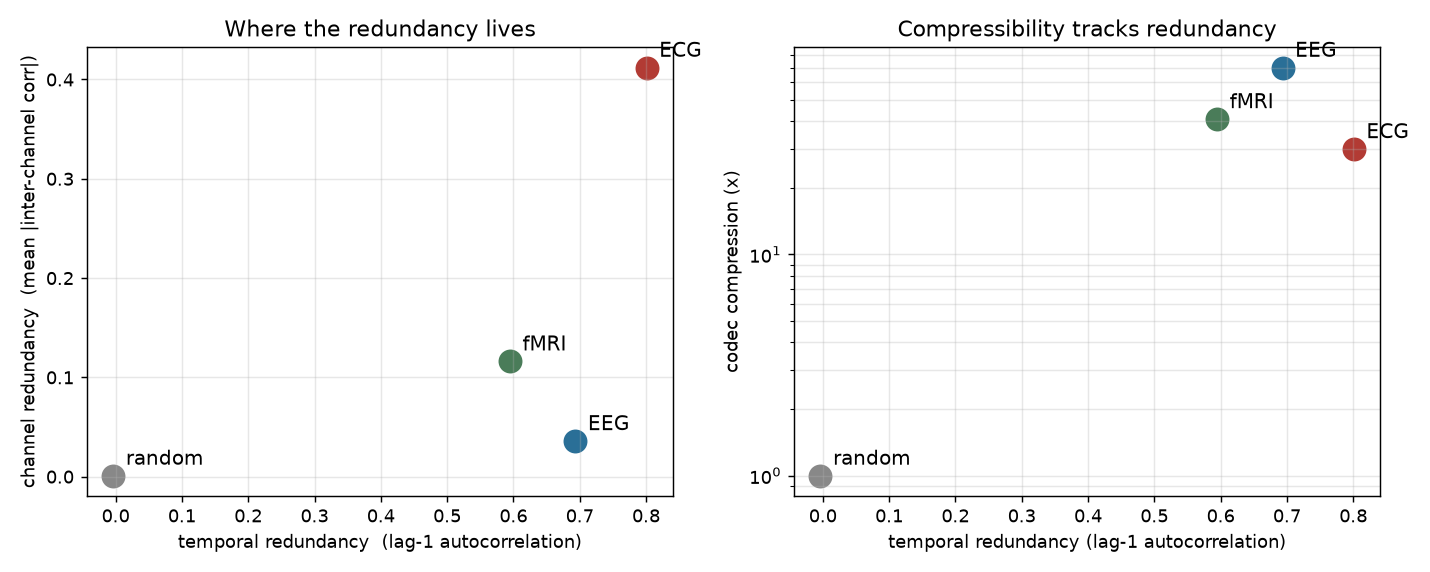
\includegraphics[width=\linewidth]{figures/redundancy_spectrum.png}
\caption{Left: where the redundancy lives (random at origin, ECG top-right). Right:
compression tracks temporal redundancy; the incompressible control sits at
$(0,1\times)$.}
\label{fig:spec}
\end{figure}

\section{Results}
\begin{table}[h]\centering\small
\begin{tabular}{llrllr}
\toprule
modality & codec (params) & comp. & fidelity & task & retained \\
\midrule
EEG & 1-D VQ (0.4M) & 70--144$\times$ & --- & CLIP retrieval & +4--11pp vs fid.\ \\
ECG & 1-D conv (1.1M) & 30$\times$ & VE 95\%, 48\,dB & 5-way dx & \textbf{98\%} \\
fMRI & 3-D VQ (0.6M) & 26$\times$ & VE 82\%, 40\,dB & VT decoding & \textbf{98--100\%} \\
fMRI & temporal-SVD (0) & 41--75$\times$ & MSE 0.06--0.09 & --- & (\S4.1) \\
HAR & 1-D conv (0.26M) & 35$\times$ & VE 93\%, 38\,dB & 6-way activity & \textbf{98\%} \\
control & --- & 1$\times$ & --- & --- & --- \\
\bottomrule
\end{tabular}
\caption{One small codec family, four modalities: task performance is preserved
under 30--300$\times$ compression.}
\label{tab:main}
\end{table}

\textbf{fMRI: the redundancy axis and the trade-off.} A per-volume codec floors at
MSE $\approx0.24$ (a single volume is high-rank in space); matching the codec to the
low-rank \emph{time} axis reaches MSE 0.089 at 75$\times$. But MSE-optimal
compression drops the low-variance multivoxel decoding signal: the codec preserving
decoding best (26$\times$, 100\% retained) is not the one with best MSE
(Fig.~\ref{fig:fmri}).

\begin{figure}[h]\centering
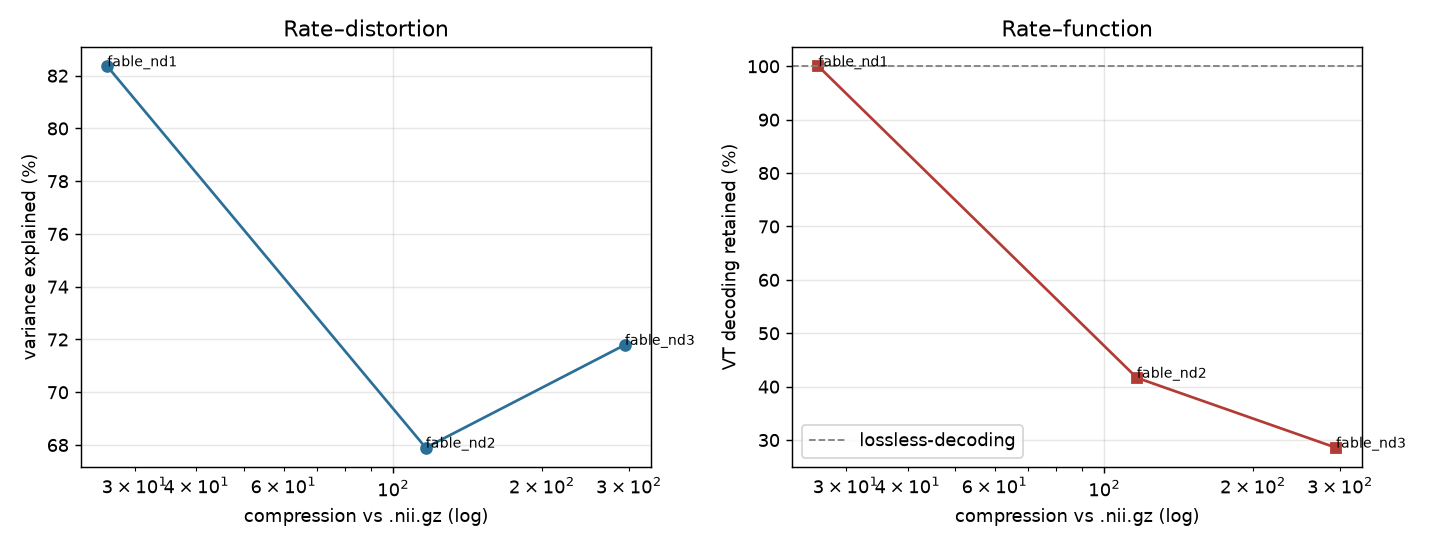
\includegraphics[width=\linewidth]{figures/fmri_rate_distortion.png}
\caption{fMRI rate--distortion (flat, near the signal ceiling) vs rate--function
(monotonic: decoding retention $29\to42\to100\%$ as rate rises).}
\label{fig:fmri}
\end{figure}

\section{Discussion \& limitations}
Compressibility is redundancy; match the codec to the redundant axis (a five-line
diagnostic); and evaluate the downstream task, not just MSE, since the two can
diverge. Limitations: some single-subject/subset evaluations; ratios at
per-modality high-fidelity operating points (not iso-fidelity); neural-codec exact
reproducibility depends on deterministic inference (the entropy layer is bit-exact).

\section*{Reproducibility}
Each experiment is a branch with a findings doc, code, checkpoints, and a one-command
test: \texttt{ecg-fable}, \texttt{fmri-fable}, \texttt{har-fable},
\texttt{redundancy-spectrum}. Datasets are public.

\end{document}
